% !TEX root = ../main.tex

% = = = = = = = = = = = = = = = = = = = = = = = = = = = = = = = = = = = = = = = = = =

\section{Introductory Remarks}

Cryptocurrencies like Bitcoin (BTC) and Ether (ETH) are marked by extreme volatility in price relative to the US dollar (USD). As decentralized finance (DeFi) services mature on Ethereum, a critical component to their success is letting users choose between holding ETH and holding a stablecoin that targets USD (or some other metric of stability) in price.

Some stablecoins work like a hypothetical vending machine~\cite{CDM20}: Alice deposits two `coins' from a volatile currency (\eg a cryptocurrency like ETH) into the machine and it returns to her two new coins---a `black' coin that is stable and a `red' coin that is even more volatile in price than the original coins Alice put in. Together, the red and black coins are equal in value to the two input coins. The machine cannot reduce overall price volatility, but it can push volatility from the black coin onto the red coin. 

Consider the following example of such a stability mechanism. An asset is chosen that is considered stable by definition (\eg the US dollar). The vending machine is implemented as a decentralized app (DApp; \aka smart contract) on a blockchain (\eg Ethereum). Alice deposits an amount of ETH worth \$1.50 USD into the DApp. The DApp references a trusted oracle service for the current ETH/USD exchange rate to enforce this. The DApp holds the ETH as a deposit for future redemption, and returns to Alice a red coin and a black coin (\eg as ERC-20 tokens). Alice can sell one or both coins. In the future, the owner of the black coin can redeem it for ETH from the DApp, and receive the equivalent of \$1.00 USD. This assumes the initial deposit of \$1.50 USD worth of ETH is still worth at least \$1.00 USD at redemption time---if not, the black coin owner receives all of the collateral. The red coin holder receives any remaining ETH after the black coin holder is paid.

The key idea is that the black coin will nearly always be worth the equivalent of \$1.00 USD. This is true when ETH/USD increases in value, stays the same, or declines moderately. Only if it declines significantly does the black coin start to experience volatility in price---its redemption value will decrease at the same rate as ETH/USD itself. For the red coin, the redemption value increases and decreases as ETH/USD itself increases and decreases, however the gains and losses are amplified. This is an overview; we return to these details below.

\paragraph{Synthetic Assets.} The red-black coin primitive can be generalized to produce black coins that match the price of any financial asset, not just a currency like the USD, simply by changing the price that the oracle references. For example, a black coin for one share of the company Apple (APPL) would use an ETH/APPL price feed (possibly constructed by bridging ETH/USD and APPL/USD prices) and otherwise be exactly the same. These black coins are `synthetic assets' because they expose the holder to the price movements of the asset but do not afford the holder any other benefits of holding the financial instrument (\eg shareholder votes or dividends for equities; physical delivery for futures; or the ability to settle a loan, or option contract on the asset). What a red coin represents in this example is less natural than for a stablecoin: it is a bet that ETH will increase in price faster than APPL.

\paragraph{Relation to Dai.} At the time of writing, the stablecoin \dai has (i) a market cap of \$800M (the largest of all non-centralized stablecoins); (ii) its parent service, Maker, locks \$1.2B worth of ETH (the third largest DeFi service, and the largest stablecoin); and (iii) it is the most supplied and most borrowed asset on the DeFi lending service Compound.\footnote{\url{https://compound.finance/markets}} \dai uses the red-black coin primitive---black coins are called \dai and a red coin is a \vault (\nee collateralized debt position or \cdp). However the system is immensely more complicated because it adds a number of features that the basic red-black coin primitive lacks: (1) interchangeability (fungibility) of black coins across multiple producers, (2) a liquidation process to incentivize red coin holders to increase the collateralized ETH as ETH/USD declines or face an auction that automatically settles a red-black pair, and (3) fees to balance supply/demand of black and red coins that are adjustable through a distributed governance. Other projects built on the red-black primitive (for both stablecoins and synthetic assets) include Synthetix's sUSD, Kava's USDX, UMA, and BitUSD. 

\paragraph{Liquidations.} The worst-case scenario for a red-black coin is a decline in the value of ETH/USD. As a primitive, red-black coins simply force the holders to take on this risk. By contrast, liquidations are the main preventative mechanism used by full-fledged systems like Dai. Liquidations are controversial: many vault holders have lost ETH due to liquidations, they require special monitoring tools (\eg \texttt{DeFiSaver.com}), any analysis includes assumptions about how humans behave and how fast market actions can be taken, and maligned incentives (\eg return DAI for ETH when ETH/DAI is in decline) can lead to economic crises and de-leveraging spirals~\cite{GPH+20,KMM20}. Liquidations failed Dai on Ethereum's `Black Thursday' event in March 2020 and required a bail-out. In this paper, red-black coins can be thought of as `Dai without liquidations.' Since liquidations have a downside, it is important to weight these against what they contribute. To understand what they contribute, we must first thoroughly understand red-black coins and their shortcomings. Further it might be possible that liquidations are not the best tool to address any shortcomings---we consider alternatives in Section~\ref{sec:taxonomy}.


\subsection{Contributions \& Related Work} We reference some financial instruments and terminology throughout the paper; we refer the reader elsewhere for full explanations of these~\cite{Har03}. Several systemization of knowledge papers cover stablecoins~\cite{PHP+19,MSS20,CDM20}. Our notion of a red-black coin is inspired by the `indirectly-backed' classification from~\cite{CDM20} \textcolor{blue}{and "exogenous collateral" type of "non-custodial" stable coins in ~\cite{klages2020stablecoins}}
. In the other two~\cite{PHP+19,MSS20}, the mechanism is described as allowing a user to `borrow' USD from themselves using their ETH as collateral---we find this perspective less intuitive. None of the three SoKs provide deep coverage, analysis, or modelling of the stability mechanism in this paper, and instead focus on surveying several different types of stablecoins and mechanisms. Maker is considered a decentralized finance (DeFi) project and it (and other DeFi projects) has been studied from orthogonal angles including attacks/measurements on governance and oracles, attacks using flash loans, and modelling liquidity crises~\cite{GRB20,GPH+20,QZLG20,KMM20}. \textcolor{blue}{In ~\cite{klages2020stablecoins}, stable coins are categorized into two main classes: custodial and non-custodial. They introduced three potential risks that may threat non-custodial stable coins (Governance, Mining, and Manipulations) and utilize a capital structure model to assess the risk under different scenarios.}



In this paper, we isolate and study the red-black coin primitive to better understand its characteristics, which seems prudent before analyzing more complex systems. We use the ETH price model from~\cite{GPH+20} to model how risky red and black coins are under different scenarios. We then examine the necessity of the extra infrastructure projects like Maker add to red-black coins---precisely what does the added complexity (\eg stability fees, liquidation, global shutdown, \etc) achieve and what are the design alternatives for the same functionality? 
\textcolor{blue}{It should be noted that in this paper we assumed that the market for red and black coins are perfectly liquid to have a simple model to analyze. In ~\cite{klages2019stability} and ~\cite{KMM20}, authors researched on the effect of supply and demand and explored the possibility of market collapse due to the feedback effects on liquidity and volatility from deleveraging effects during crises. These works assumed liquidation process as a building block of non-collateral stable coins which we argued in this paper.}

\textcolor{blue}{In addition to our work, there are other two coin solutions to implement stablecoins. For instance, ~\cite{DUOnet}  proposed a new model in which the stable coin is similar to the coupon bond in traditional finance and the other riskier coin is similar to leveraged positions. They used traditional option theory models to analyze their system.}

%None of the papers include a design landscape for 'indirectly-backed' stable coins, which could help future designs in this category. We also employ a quantitative finance method and run different experiments to clarify how risky these stable coins are. 

% = = = = = = = = = = = = = = = = = = = = = = = = = = = = = = = = = = = = = = = = = =

\section{Financial Characteristics}


\begin{figure}[t]
    \centering
        \subfloat[A red coin, a black coin, and ETH equivalent to \$0.50.]{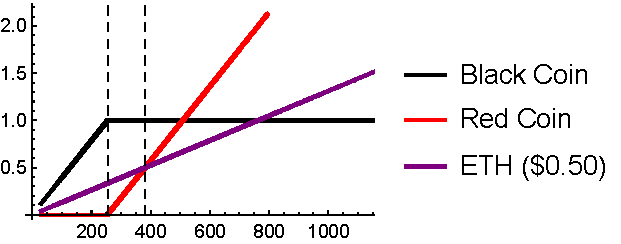
\includegraphics[height=2.5cm]{figures/price1.pdf}}
        \qquad
        \subfloat[A red coin, ETH equivalent to \$1.50, and a portfolio of a red coin and \$0.94.]{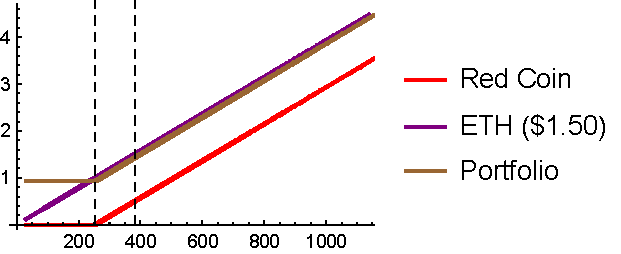
\includegraphics[height=2.5cm]{figures/price2.pdf}}
    \caption{Redemption value in USD (y-axis) as the price of ETH (x-axis) changes. \label{fig:price1} \label{fig:price2}}
\end{figure}

In this section, we answer questions about the financial characteristics of the red-black primitive. Consider a black coin that targets \$1 USD when 1 ETH is \$381.56 USD, and the DApp holds 0.00393126 ETH (worth \$1.5 USD).  Assume for now that (i) a red-black coin is a (non-fungible) contract between two individuals, and (ii) no one intervenes when ETH/USD declines enough that black coins starts to lose value (no liquidations). Figure~\ref{fig:price1}(a) shows how much a black coin is worth (y-axis) as the price of ETH varies (x-axis). The starting point (\$381.56 USD) is marked and if the price of ETH increases (rightward), the black coin is always worth \$1. If the value of ETH decreases (leftward), the black coin is still stable until the value of ETH hits \$254.37 (marked)---at this point, 0.00393126 ETH starts to become worth less than \$1 and the black coin `breaks the buck.'

Figure~\ref{fig:price1}(a) also shows the redemption value of a red coin. When created, a red coin is redeemable for \$0.50 USD. A user with \$0.50 USD can choose between purchasing a red coin or purchasing ETH (also shown). In both cases, the user profits when ETH increases and loses when ETH decreases in price. However the slope of red coin is greater. This indicates it is a \emph{leveraged} position in ETH.  

% = = = = = = = = = = = = = = = = = = = = = = = = = = = = = = = = = = = = = = = = = =

\subsection{How much should you pay for a black coin?}

Consider a black coin that is purchased today when ETH is \$381.56 USD. How much will it be worth in 100 days? In most future worlds, the black coin will be worth \$1. In some future worlds (when ETH is worth less than \$254.37), the black coin will break the buck. But even here, it takes a `haircut' on value as opposed to being worthless (\eg it can be redeemed for, say, \$0.90). 

\begin{figure}[t]
    \centering
        \subfloat[Price of ETH in USD (y-axis) over number of days (x-axis).]{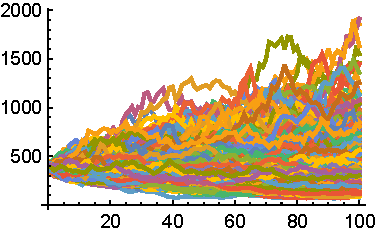
\includegraphics[width=0.4\columnwidth]{figures/mc.pdf}}
        \qquad
        \subfloat[Histogram of final price of ETH in USD (x-axis).]{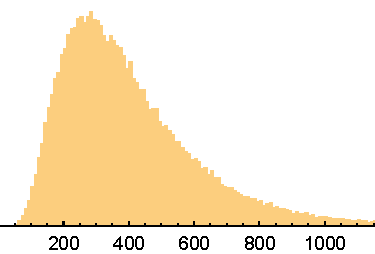
\includegraphics[width=0.4\columnwidth]{figures/histro.pdf}\label{fig:histro}}
    \caption{ETH/USD Monte Carlo simulation results. \label{fig:sim}}
\end{figure}

The \textcolor{blue}{Average value of a black coin for different possible outcomes} can be estimated if we have a statistical model for ETH price movements. In finance, many statistical models have been proposed for many assets. Pricing ETH remains an open research problem. Until future research from the finance community advocates for the most appropriate model, we will sketch in some concrete numbers using Geometric Brownian Motion (GBM), which underlies the Black-Scholes model for pricing options~\cite{BS73} and has been used for ETH in other work~\cite{GPH+20}. We omit the details of the model itself (covered in nearly every  financial textbook~\cite{Sey09}). We fit the model to the historical `closing' prices of ETH for 1000 days prior to 18 Sept 2020\footnote{CoinGecko API: \url{https://api.coingecko.com}} and obtain $\mu=0.000744754$ (an upward drift in price over time) and $\sigma=0.0524172$ (a measure of volatility). If we simulate the next 100 days using Monte Carlo, we obtain the results in Figure~\ref{fig:sim}. For the parameters of this example, the \textcolor{blue}{Average value} of the black coin is \$0.94 USD \textcolor{blue}{at the maturity date}. Our model can be adjusted for the initial price, over-collateralization ratio (section ~\ref{sec:redchar}), and days until redemption. It is available in Python and Mathematica.\footnote{GitHub: URL omitted for anonymity.} 

As shown in Figure~\ref{fig:sim}\subref{fig:histro}, the expected return is log-normal. When we model more than 100 days, the variance increases and the \textcolor{blue}{Average} redemption value of a black coin decreases: \$0.94 USD after 100 days, \$0.85 USD after 200 days, and \$0.80 after 1 year. This does not mean the black coin is worth less over time, it means the risk it falls out-of-the-money increases the more time you give it. 

% = = = = = = = = = = = = = = = = = = = = = = = = = = = = = = = = = = = = = = = = = =

\subsection{Why would you want a red coin?}
\label{sec:redchar}

While a stablecoin has utility to the holder, it is less clear what the utility of a red coin is. A red coin is a \textit{leveraged} position in ETH, which means that both gains and losses are amplified---compare the slope of the red coin value with a \$0.50 ETH investment at the same starting point (\$381.56 USD) in Figure~\ref{fig:price1}(a). Leverage is popular with investors. Investing in a red coin is equivalent to investing \$0.50 along with borrowing $2\times\$0.50$ in ETH (\ie 3:1 leverage). If the over-collateralization ratio is decreased from 1.50 to 1.10, then leverage for the red coin increases to 11:1. However, the black coin becomes riskier and its 100-day \textcolor{blue}{Average} value drops from \$0.94 to \$0.86. For a \$2.00 collateralization, red coin leverage is 2:1, and the black coin \textcolor{blue}{Average} value is \$0.98. 

Speculators seek out red coins but what about a user that wants to hold ETH without any leverage? She seemingly has no interest in red (or black) coins. Consider two scenarios: (a) she holds \$1.50 worth of ETH; and (b) she takes her \$1.50 worth of ETH, issues and sells a black coin (\eg for \$0.97 USD), and holds the red coin. She actually has a small portfolio of a red coin and close to \$1 USD. The redemption value of (a) and (b) are depicted in Figure~\ref{fig:price2}(b), along with the red coin by itself. The portfolio is actually an attractive investment---she has `insurance' against catastrophic loss during a devaluation of ETH for a small fixed `fee'---the \$0.03 USD difference between what she received for the black coin (\$0.94) and what the DApp pays out to the black coin holder (\$1.00). Additionally, she produced a stable black coin, which has external benefit to the decentralized economy. 

%With decentralized lending protocols (\eg Compound), red coins can earn interest with the same mechanism used for ETH, and the USD can also earn a return.

% = = = = = = = = = = = = = = = = = = = = = = = = = = = = = = = = = = = = = = = = = =

\section{Research Agenda: Extending Red-Black Coins}
\label{sec:taxonomy}

Red-black coins are primitives. Before deploying them, other aspects of their design should to be considered. Design decisions include the maturity/redemption policy, how to make black and red coins fungible, and interventions to prevent the black coin from breaking the buck. One path through the decision tree leads to a design like \dai, however there are many other decisions that could result in very different stablecoins that have not been thoroughly explored by academics or the DeFi community to our knowledge. We do not propose a specific alternative but see our contribution as setting a research agenda. 

%The purpose of this section is to emphasize that \dai is one set of reasonable decisions but there are many alternative designs that have not been (to our knowledge) explored.

% = = = = = = = = = = = = = = = = = = = = = = = = = = = = = = = = = = = = = = = = = =

\subsection{Fungibility}

Assume Alice creates a red/black coin, selling the red coin to Carol. Later, Bob creates a red/black coin, selling the red coin to David. Alice's black coin is not identical to Bob's black coin. Because they were created at different times, the ETH/USD exchange rate is different, and thus the  amount of collateral in ETH in the DApp will be different. The more collateral, the more a black coin is worth (recall Section~\ref{sec:redchar}). Such coins are not interchangeable or \textit{fungible} which adds effort to valuation and exchange. 

One design option is to \textbf{(1) forgo fungibility} and have each coin pair be its own individual contract between two counter-parties (\aka over-the-counter (OTC) contracts). This is the difference between, say, a forward and futures contract~\cite{Har03}. A second option is to \textbf{(2) pool the collateral} of the red coins so that each black coin is a claim against the pool. A pool can be unfair: the losses are democratized to all black coin holders. When pooled, Alice might obtain a black coin before an ETH/USD price bubble; all the black coins issued during the rising bubble are backed by significantly less collateral and when the bubble bursts (consider the case that it reverts to the pre-bubble price), the pool could become under-collateralized, impacting Alice. Had Alice used an OTC contract instead, her red coin would acquire and lose value with the bubble but not be under-collaterialized after bursting. 

A third option is to additionally offer \textbf{(3) red coin fungibility}. Since red coins have variable collateral (based on when they were created), two conditions need to be added to its transfer function: (i) red coins with less than a specified collateral are not transferable, and (ii) red coins with more than the specified collateral will transfer the surplus to the seller’s address while transferring it. While this is not possible with vaults in \dai currently, it seems feasible to add.
	
% = = = = = = = = = = = = = = = = = = = = = = = = = = = = = = = = = = = = = = = = = =

\subsection{Redemption}
\label{sec:maturity}

A policy for redeeming the collateralized ETH is the next design decision. Note that the DApp can autonomously distribute the collateral without the participation of the red or black coin holder, however someone needs to trigger a function call against the DApp to finalize the process.

 Red-black coins could \textbf{(1) mature on a pre-specified date} (\eg the first day of a specified month). At any given time, red/black coins in circulation would have one of a few different expiration dates, while still allowing some degree of fungibility. Coin holders would shorten or extend their coins by trading for a coin with a different maturity date. This is precisely how futures  mature~\cite{Har03}, and yTokens are based on the same principle~\cite{RoNi20}. After maturity, the DApp would lock all transfer functions and only allow withdrawal by the coin holders. The first to ask for a withdrawal would trigger the DApp to look up the ETH/USD price as of the maturity date and split the collateral accordingly. 

Alternatively, red-black coins could be redeemed at any time \textbf{(2) on demand by the black coin holder}, or \textbf{(3) red coin holder}, \textbf{(4) either}, or \textbf{(5) both}. Options (in the US style) work on the principal of (2) or (3)~\cite{Har03,Sey09}. Allowing either to redeem is unlike anything we could find in traditional finance---we speculate it would add uncertainty without any clear gain. Requiring both to agree to redemption could be done by agreement, or (consistent with futures contracts~\cite{Har03}), a red coin holder could acquire a (fungible) black coin and redeem the (netted-out) pair.

% = = = = = = = = = = = = = = = = = = = = = = = = = = = = = = = = = = = = = = = = = = = = = = = = = =

\subsection{Under-collateralization}

When the ETH/USD exchange rate drops enough that under-collateralization is possible, the system could \textbf{(1) do nothing} and let the black coin holder price the risk of this into the coin. If the design attempts further mitigation, the DApp could operate like a margin trading account and require red coin holders to top-up their collateral. If they do not, it is \textbf{(2) liquidated} (\eg sold by auction for black coins). The challenge is incentivizing users to sell USD-pegged black coins for ETH when ETH/USD is in decline (a counter-cyclic investment). In \dai, because collateral is pooled, liquidation is essential because under-collateralized red coins hurt all black coin holders. When collateral is not pooled, liquidation is useless for black coin holders because both ETH and black coins decrease in value at the same rate (recall Figure~\ref{fig:price1}) so it is simpler to do nothing.

Liquidation does not incentivize topped-up collateral unless it is accompanied by a \textbf{(3) punishment} (otherwise red coin holders might try to buy their liquidated assets from themselves at a discount). Beyond charging a fee, a stablecoin system might also withhold rewards (some systems used a secondary token for providing governance and providing rewards) or block red coin transfers until collateral is restored. In traditional financial markets, it is also the case that a trader's margin is inadequate to settle their account, they are still legally liable for the difference. A stablecoin accompanied by a \textbf{(4) reputation system} could mandate that red coin holders settle any obligation, however the potential loses for a red coin holder becomes unbound. A different approach is to obtain \textbf{(5) insurance} or financial coverage for the event of a decline in ETH/USD. This could be actual insurance, whether decentralized or from a traditional brokerage, or an offsetting financial investment that hedges the currency exchange risk. %This is similar to Abra. %Insurance or hedging could be done for a pool of red/black coins, or more simply, it could be done on the individual level (a stablecoin would consist of one black coin and an option to sell for \$1 USD).  

The last approach is \textbf{(6) bail out} any losses through sales of a secondary token. This was used recently by Maker for \dai holders when its normal procedures of (2) and (3) were not adequate for dealing with a sharp, unexpected decline in the price of ETH on 12 Mar 2020 (`black Thursday'). While the auction was successful and recollateralized the pool, it cannot be guaranteed that minting new tokens will be adequate for offsetting any incurred debt. This event also exposed the lack of understanding and underestimation of risk by many vault (\ie red coin) holders who faced losses under (3), and raises the question of whether a system should be designed that is more forgiving to red coin holders in turbulent markets.%, especially since their financial position enables the issuance of a stablecoin. 

% = = = = = = = = = = = = = = = = = = = = = = = = = = = = = = = = = = = = = = = = = = = = = = = = = =

\subsection{Autonomy} 

A design based on the red-black coin primitive that is OTC and does not liquidate is entirely autonomous. It can be instantiated in a DApp and operate without human intervention. While black coins are price-stable under most market conditions, traders who are time-sensitive may forgo obtaining a good price in order to trade quickly. This particularly is influential for stablecoins which provide a low-friction avenue in and out of speculative positions on the price of ETH. Since red and black coins are issued in the same proportion, supply/demand imbalances between them could also add volatility to the black coin price. This could potentially be addressed in the design. 

A non-interventionist approach would let the red and black coin price \textbf{(1) float freely}. This avoids adding complexity to the design---in fact, a design goal might be to design a system that traders can easily understand and grasp the risk of. This could thwart potential lawsuits, such as a recent class action suit against \dai.\footnote{CoinDesk: \url{https://t.co/iJET1JGJib}} An alternative is to further stabilize prices by \textbf{(2) setting rates and fees} at various points in the system. For example, if black coin holders can redeem at any time, a fee could be charged to the black coin holder and paid to the red coin holder. If redemption requires both a red and black coin, the fee could be collected by the DApp. This principle is used by central banks for targeting interest rates, and is used in Maker to control the spot market for \dai. It is a struggle to set fees in the context of a decentralized and autonomous organization---while allowing decisions to be voted on is a first step, it does not guarantee that token holders are independent, informed, and not unduly influenced by the `expert' recommendations. 

% = = = = = = = = = = = = = = = = = = = = = = = = = = = = = = = = = = = = = = = = = = = = = = = = = =
% = = = = = = = = = = = = = = = = = = = = = = = = = = = = = = = = = = = = = = = = = = = = = = = = = =
% = = = = = = = = = = = = = = = = = = = = = = = = = = = = = = = = = = = = = = = = = = = = = = = = = =

\section{Concluding Remarks}

In this paper, we distil complex stablecoin systems into one of their core primitives, the red-black coin and provide a detailed study of its characteristics and possible extensions. It would be useful to have research results on the most suitable financial model for the ETH/USD price rate (\eg drift-diffusion or GARCH) for us to use in work like this paper. Future work could also examine the benefits of building a \dai alternative, still based on red-black coins but using different design parameters. Two examples that seem interesting are: (a) a more understandable system that reduces the amount of intervention, and (b) a system with fungible red coins that can be traded freely. Finally, while our paper answers the question of how much you should pay for a black coin, the analysis is much more complicated for \dai---with pooled collateral, liquidation, and bailouts, \dai is less risky than a simple black coin but the risk that these countermeasures systemically fail is not zero.

